% Practice Test 02 — Oklahoma Edition
% Questions: 30 (22 MC + 8 SA)
% Generated by scripts/generate_practice_tests.py

\begin{practiceQuestion}{1-3-q30}{gsa}
\begin{questionText}
The table shows a proportional relationship between minutes and laps completed. Find $k$ and determine how many laps are completed in $15$ minutes.

\begin{center}
\begin{tabular}{|c|c|}
\hline
\textbf{Minutes ($x$)} & \textbf{Laps ($y$)} \\ \hline
$4$ & $3$ \\ \hline
$8$ & $6$ \\ \hline
$12$ & $9$ \\ \hline
$15$ & $?$ \\ \hline
\end{tabular}
\end{center}
\end{questionText}
\correctAnswer{$k = 0.75$; $11.25$ laps in $15$ minutes}
\explanation{$k = \frac{3}{4} = 0.75$. For $15$ minutes: $y = 0.75 \times 15 = 11.25$ laps.}
\end{practiceQuestion}

\begin{practiceQuestion}{1-6-q07}{mc}
\begin{questionText}
On a map, $3$ cm represents $24$ km. How far apart are two towns that are $8$ cm apart on the map?
\end{questionText}
\choiceA{$48$ km}
\choiceB{$56$ km}
\choiceC{$64$ km}
\choiceD{$72$ km}
\correctAnswer{C}
\explanation{$\frac{3}{24} = \frac{8}{d}$. Cross-multiply: $3d = 192$, so $d = 64$ km.}
\end{practiceQuestion}

\begin{practiceQuestion}{1-7-q25}{sa}
\begin{questionText}
A model rocket is $40$ cm tall and the real rocket is $120$ m tall. How many centimeters on the model represent $1$ meter on the real rocket?
\end{questionText}
\correctAnswer{$\frac{1}{3}$ cm}
\explanation{Scale: $12{,}000 \div 40 = 300$. So $1$ m on the real rocket is $100 \div 300 = \frac{1}{3}$ cm on the model.}
\end{practiceQuestion}

\begin{practiceQuestion}{2-1-q13}{mc}
\begin{questionText}
Which proportion can be used to find $30\%$ of $90$?
\end{questionText}
\choiceA{$\dfrac{n}{90} = \dfrac{30}{100}$}
\choiceB{$\dfrac{30}{n} = \dfrac{90}{100}$}
\choiceC{$\dfrac{90}{n} = \dfrac{30}{100}$}
\choiceD{$\dfrac{n}{100} = \dfrac{30}{90}$}
\correctAnswer{A}
\explanation{The part $n$ is over the whole $90$, and the percent $30$ is over $100$: $\frac{n}{90} = \frac{30}{100}$.}
\end{practiceQuestion}

\begin{practiceQuestion}{2-4-q06}{mc}
\begin{questionText}
A book costs $\$14$, and sales tax is $7\%$. What is the total?
\end{questionText}
\choiceA{$\$14.07$}
\choiceB{$\$14.70$}
\choiceC{$\$14.98$}
\choiceD{$\$15.40$}
\correctAnswer{C}
\explanation{Tax: $14 \times 0.07 = \$0.98$. Total: $14 + 0.98 = \$14.98$.}
\end{practiceQuestion}

\begin{practiceQuestion}{2-7-q10}{mc}
\begin{questionText}
A weather forecast predicted $3$ inches of rain. The actual rainfall was $2.5$ inches. What is the percent error?
\end{questionText}
\choiceA{$0.5\%$}
\choiceB{$10\%$}
\choiceC{$16.7\%$}
\choiceD{$20\%$}
\correctAnswer{D}
\explanation{$\frac{|3 - 2.5|}{2.5} \times 100 = \frac{0.5}{2.5} \times 100 = 20\%$.}
\end{practiceQuestion}

\begin{practiceQuestion}{2-8-q30}{gsa}
\begin{questionText}
The bar graph shows the annual fees at two banks and the annual interest earned on a $\$2{,}000$ deposit. Which bank is the better deal, and how much more do you gain (or save) per year by choosing it?

\begin{center}
\begin{tikzpicture}[scale=0.6]
  \draw[thick,->] (0,0) -- (0,6) node[above] {\$};
  \draw[thick,->] (0,0) -- (10,0);
  \foreach \y/\label in {0/0, 1/10, 2/20, 3/30, 4/40, 5/50} {
    \draw (-0.1,\y) -- (0.1,\y);
    \node[left] at (-0.15,\y) {\footnotesize \$\label};
  }
  % Bank P - Fee
  \fill[funRed!60] (0.5,0) rectangle (1.8,3.6);
  \node[below] at (1.15,-0.1) {\footnotesize Fee};
  \node[above] at (1.15,3.6) {\footnotesize \$36};
  % Bank P - Interest
  \fill[funBlue!60] (2.2,0) rectangle (3.5,4);
  \node[below] at (2.85,-0.1) {\footnotesize Interest};
  \node[above] at (2.85,4) {\footnotesize \$40};
  \node[below] at (2,-.8) {\footnotesize Bank P};

  % Bank Q - Fee
  \fill[funRed!60] (5.5,0) rectangle (6.8,1.2);
  \node[below] at (6.15,-0.1) {\footnotesize Fee};
  \node[above] at (6.15,1.2) {\footnotesize \$12};
  % Bank Q - Interest
  \fill[funBlue!60] (7.2,0) rectangle (8.5,3);
  \node[below] at (7.85,-0.1) {\footnotesize Interest};
  \node[above] at (7.85,3) {\footnotesize \$30};
  \node[below] at (7,-.8) {\footnotesize Bank Q};
\end{tikzpicture}
\end{center}
\end{questionText}
\correctAnswer{Bank Q by $\$14$}
\explanation{Bank P net: $40 - 36 = \$4$ gain. Bank Q net: $30 - 12 = \$18$ gain. Bank Q is better by $18 - 4 = \$14$.}
\end{practiceQuestion}

\begin{practiceQuestion}{3-1-q01}{mc}
\begin{questionText}
What is the opposite of $-6$?
\end{questionText}
\choiceA{$-6$}
\choiceB{$0$}
\choiceC{$6$}
\choiceD{$\frac{1}{6}$}
\correctAnswer{C}
\explanation{The opposite of a negative number is positive. The opposite of $-6$ is $6$ because both are $6$ units from $0$.}
\end{practiceQuestion}

\begin{practiceQuestion}{4-1-q23}{sa}
\begin{questionText}
A cell phone plan charges $c$ cents per minute. Write an expression for the cost of a $15$-minute call in dollars.
\end{questionText}
\correctAnswer{$\frac{15c}{100}$ or $0.15c$}
\explanation{$15$ minutes at $c$ cents each is $15c$ cents. To convert to dollars, divide by $100$: $\frac{15c}{100} = 0.15c$.}
\end{practiceQuestion}

\begin{practiceQuestion}{4-2-q15}{mc}
\begin{questionText}
Simplify $10 - 3x + 5x - 4$.
\end{questionText}
\choiceA{$8x + 6$}
\choiceB{$-8x + 6$}
\choiceC{$2x + 6$}
\choiceD{$2x - 6$}
\correctAnswer{C}
\explanation{Combine variable terms: $-3x + 5x = 2x$. Combine constants: $10 - 4 = 6$. Result: $2x + 6$.}
\end{practiceQuestion}

\begin{practiceQuestion}{5-3-q21}{sa}
\begin{questionText}
Solve $5(2x - 3) = 35$.
\end{questionText}
\correctAnswer{$x = 5$}
\explanation{Divide by $5$: $2x - 3 = 7$. Add $3$: $2x = 10$. Divide by $2$: $x = 5$. Check: $5(2(5) - 3) = 5(7) = 35$ \checkmark.}
\end{practiceQuestion}

\begin{practiceQuestion}{5-4-q05}{mc}
\begin{questionText}
Solve $\dfrac{2x}{5} - 1 = 3$.
\end{questionText}
\choiceA{$x = 5$}
\choiceB{$x = 10$}
\choiceC{$x = 4$}
\choiceD{$x = 20$}
\correctAnswer{B}
\explanation{Add $1$: $\frac{2x}{5} = 4$. Multiply by $5$: $2x = 20$. Divide by $2$: $x = 10$. Check: $\frac{2(10)}{5} - 1 = 4 - 1 = 3$ \checkmark.}
\end{practiceQuestion}

\begin{practiceQuestion}{5-5-q09}{mc}
\begin{questionText}
A student solved $-2x + 8 > 14$ and wrote $x > -3$. What error did the student make?
\end{questionText}
\choiceA{Forgot to subtract $8$}
\choiceB{Divided by $2$ instead of $-2$}
\choiceC{Forgot to flip the inequality sign}
\choiceD{Added $8$ instead of subtracting}
\correctAnswer{C}
\explanation{Correct steps: subtract $8$ → $-2x > 6$. Divide by $-2$ and flip: $x < -3$. The student forgot to flip.}
\end{practiceQuestion}

\begin{practiceQuestion}{5-6-q12}{mc}
\begin{questionText}
Solve $2x - 1 < 7$ and describe the graph.
\end{questionText}
\choiceA{Open circle at $4$, shade left}
\choiceB{Closed circle at $4$, shade left}
\choiceC{Open circle at $3$, shade left}
\choiceD{Open circle at $4$, shade right}
\correctAnswer{A}
\explanation{Add $1$: $2x < 8$. Divide by $2$: $x < 4$. Open circle at $4$, shade left.}
\end{practiceQuestion}

\begin{practiceQuestion}{6-2-q04}{mc}
\begin{questionText}
A drawing uses $1$ cm $= 3$ m. It is redrawn at $1$ cm $= 9$ m. A room that is $12$ cm on the original becomes how long?
\end{questionText}
\choiceA{$4$ cm}
\choiceB{$12$ cm}
\choiceC{$36$ cm}
\choiceD{$108$ cm}
\correctAnswer{A}
\explanation{Scale ratio: $\frac{3}{9} = \frac{1}{3}$. New length: $12 \times \frac{1}{3} = 4$ cm.}
\end{practiceQuestion}

\begin{practiceQuestion}{6-3-q16}{mc}
\begin{questionText}
A parallelogram has side lengths $5$ cm and $8$ cm. How many different parallelograms can be drawn?
\end{questionText}
\choiceA{None}
\choiceB{Exactly one}
\choiceC{Exactly two}
\choiceD{More than one}
\correctAnswer{D}
\explanation{Two side lengths of a parallelogram do not fix the angles. The shape can be a rectangle, a rhomboid, or anything in between. Many different parallelograms are possible.}
\end{practiceQuestion}

\begin{practiceQuestion}{6-4-q26}{gmc}
\begin{questionText}
The diagram shows a triangle with the given angle measures. Is this a valid triangle?

\begin{center}
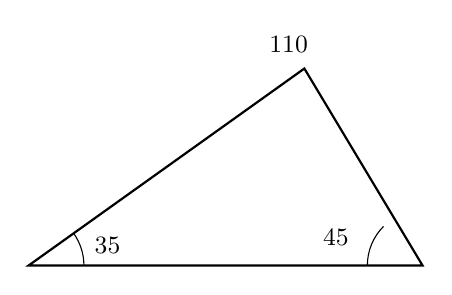
\begin{tikzpicture}[scale=1]
  \draw[thick] (0,0) -- (5,0) -- (3.5,2.5) -- cycle;
  \draw (0.7,0) arc[start angle=0,end angle=35,radius=0.7];
  \node at (1.0,0.25) {\small $35°$};
  \draw (4.3,0) arc[start angle=180,end angle=135,radius=0.7];
  \node at (3.9,0.35) {\small $45°$};
  \node at (3.3,2.8) {\small $110°$};
\end{tikzpicture}
\end{center}
\end{questionText}
\choiceA{Yes, because $35 + 45 + 110 = 190$}
\choiceB{Yes, because all angles are positive}
\choiceC{No, because the angles sum to $190°$ instead of $180°$}
\choiceD{No, because one angle is greater than $90°$}
\correctAnswer{C}
\explanation{$35 + 45 + 110 = 190 \neq 180$. Triangle angles must sum to exactly $180°$, so this triangle is not valid.}
\end{practiceQuestion}

\begin{practiceQuestion}{6-5-q07}{mc}
\begin{questionText}
A triangular prism is sliced with a cut parallel to its triangular base. What is the cross-section?
\end{questionText}
\choiceA{A rectangle}
\choiceB{A triangle congruent to the base}
\choiceC{A smaller triangle}
\choiceD{A trapezoid}
\correctAnswer{B}
\explanation{A cut parallel to the base of a prism always produces a shape congruent (same size and shape) to the base. For a triangular prism, this is a triangle identical to the base.}
\end{practiceQuestion}

\begin{practiceQuestion}{6-6-q28}{gmc}
\begin{questionText}
In the diagram, angle $1$ and angle $2$ are complementary. Angle $1$ measures $53°$. What is angle $2$?

\begin{center}
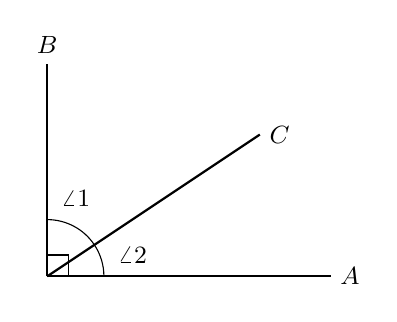
\begin{tikzpicture}[scale=0.9]
  \draw[thick] (0,0) -- (4,0);
  \draw[thick] (0,0) -- (0,3);
  \draw[thick] (0,0) -- (3,2);
  \draw (0.8,0) arc[start angle=0,end angle=34,radius=0.8];
  \node at (1.2,0.3) {\small $\angle 2$};
  \draw (0,0.8) arc[start angle=90,end angle=34,radius=0.8];
  \node at (0.4,1.1) {\small $\angle 1$};
  \node[right] at (4,0) {\small $A$};
  \node[above] at (0,3) {\small $B$};
  \node[right] at (3,2) {\small $C$};
  % Right angle mark
  \draw (0.3,0) -- (0.3,0.3) -- (0,0.3);
\end{tikzpicture}
\end{center}
\end{questionText}
\choiceA{$27°$}
\choiceB{$37°$}
\choiceC{$53°$}
\choiceD{$127°$}
\correctAnswer{B}
\explanation{The two angles together form a right angle ($90°$). $90° - 53° = 37°$.}
\end{practiceQuestion}

\begin{practiceQuestion}{7-4-q29}{gsa}
\begin{questionText}
Find the area of the shaded L-shaped figure shown below. Each square on the grid is $1$ ft by $1$ ft.

\begin{center}
\begin{tikzpicture}[scale=0.5]
  \draw[step=1,gray!30,thin] (0,0) grid (8,8);
  \fill[funBlue!20] (1,1) -- (7,1) -- (7,5) -- (4,5) -- (4,7) -- (1,7) -- cycle;
  \draw[thick,funBlue] (1,1) -- (7,1) -- (7,5) -- (4,5) -- (4,7) -- (1,7) -- cycle;
  \node[below] at (4,0.8) {$6$};
  \node[right] at (7.2,3) {$4$};
  \node[above] at (2.5,7.2) {$3$};
  \node[left] at (0.8,4) {$6$};
\end{tikzpicture}
\end{center}
\end{questionText}
\correctAnswer{$30$ ft$^2$}
\explanation{Bottom rectangle: $6 \times 4 = 24$ ft$^2$. Top-left rectangle: $3 \times 2 = 6$ ft$^2$. Total: $24 + 6 = 30$ ft$^2$.}
\end{practiceQuestion}

\begin{practiceQuestion}{7-5-q12}{mc}
\begin{questionText}
A storage box is in the shape of a cube with side $12$ inches. What is its surface area?
\end{questionText}
\choiceA{$144$ in$^2$}
\choiceB{$432$ in$^2$}
\choiceC{$864$ in$^2$}
\choiceD{$1728$ in$^2$}
\correctAnswer{C}
\explanation{$SA = 6s^2 = 6 \times 144 = 864$ in$^2$.}
\end{practiceQuestion}

\begin{practiceQuestion}{7-6-q28}{gmc}
\begin{questionText}
A triangular prism is shown below. What is its volume?

\begin{center}
\begin{tikzpicture}[scale=0.35]
  % Front triangle
  \fill[funBlue!10] (0,0) -- (8,0) -- (4,5) -- cycle;
  \draw[thick,funBlue] (0,0) -- (8,0) -- (4,5) -- cycle;
  % Back triangle
  \fill[funBlue!20] (3,2) -- (11,2) -- (7,7) -- cycle;
  \draw[thick,funBlue] (3,2) -- (11,2) -- (7,7) -- cycle;
  % Connecting edges
  \draw[thick,funBlue] (0,0) -- (3,2);
  \draw[thick,funBlue] (8,0) -- (11,2);
  \draw[thick,funBlue] (4,5) -- (7,7);
  % Labels
  \draw[thick,funRed,<->] (0,-0.8) -- (8,-0.8);
  \node[below,funRed] at (4,-0.8) {$8$ m};
  \draw[dashed,gray] (4,0) -- (4,5);
  \node[left,funRed] at (3.8,2.5) {$5$ m};
  \node[right,funRed] at (11.2,4.5) {$12$ m};
\end{tikzpicture}
\end{center}
\end{questionText}
\choiceA{$120$ m$^3$}
\choiceB{$240$ m$^3$}
\choiceC{$480$ m$^3$}
\choiceD{$96$ m$^3$}
\correctAnswer{B}
\explanation{$B = \frac{1}{2} \times 8 \times 5 = 20$ m$^2$. $V = 20 \times 12 = 240$ m$^3$.}
\end{practiceQuestion}

\begin{practiceQuestion}{8-1-q13}{mc}
\begin{questionText}
A manager surveys every $20$th customer who enters a store. This is an example of:
\end{questionText}
\choiceA{A voluntary sample}
\choiceB{A convenience sample}
\choiceC{A systematic sample}
\choiceD{A biased sample}
\correctAnswer{C}
\explanation{Selecting every $n$th member is called systematic sampling.}
\end{practiceQuestion}

\begin{practiceQuestion}{8-3-q10}{mc}
\begin{questionText}
Group A: median $85$, IQR $8$. Group B: median $80$, IQR $20$. How do the groups compare?
\end{questionText}
\choiceA{Group A is higher and more consistent}
\choiceB{Group A is higher and less consistent}
\choiceC{Group B is higher and more consistent}
\choiceD{Both groups are equally consistent}
\correctAnswer{A}
\explanation{Group A has a higher median ($85$ vs.\ $80$) and a smaller IQR ($8$ vs.\ $20$), meaning it is higher and more tightly clustered.}
\end{practiceQuestion}

\begin{practiceQuestion}{8-4-q08}{mc}
\begin{questionText}
Class P: mean $70$, median $72$, range $15$, MAD $4$.
Class Q: mean $68$, median $67$, range $35$, MAD $9$.
Which class has more consistent scores?
\end{questionText}
\choiceA{Class P}
\choiceB{Class Q}
\choiceC{Both are equally consistent}
\choiceD{Cannot be determined}
\correctAnswer{A}
\explanation{Class P has smaller range ($15$ vs.\ $35$) and smaller MAD ($4$ vs.\ $9$), meaning its scores are more tightly clustered.}
\end{practiceQuestion}

\begin{practiceQuestion}{8-5-q06}{mc}
\begin{questionText}
Using the stem-and-leaf plot in the previous question, what is the smallest data value?
\end{questionText}
\choiceA{$42$}
\choiceB{$4$}
\choiceC{$2$}
\choiceD{$45$}
\correctAnswer{A}
\explanation{The first stem is $4$ and the first leaf is $2$, so the smallest value is $42$.}
\end{practiceQuestion}

\begin{practiceQuestion}{8-7-q29}{gsa}
\begin{questionText}
The double bar graph compares test scores for two classes over three tests.

\begin{center}
\begin{tikzpicture}[scale=0.5]
  \draw[thick,->] (0,0) -- (0,6.5) node[above]{\small Average Score};
  \draw[thick,->] (0,0) -- (8.5,0);
  % Test 1
  \fill[funBlue!70] (0.5,0) rectangle (1.5,4);
  \fill[funOrange!70] (1.6,0) rectangle (2.6,3.5);
  \node[below,font=\tiny] at (1.55,0) {Test 1};
  % Test 2
  \fill[funBlue!70] (3.2,0) rectangle (4.2,4.5);
  \fill[funOrange!70] (4.3,0) rectangle (5.3,5);
  \node[below,font=\tiny] at (4.25,0) {Test 2};
  % Test 3
  \fill[funBlue!70] (5.9,0) rectangle (6.9,5);
  \fill[funOrange!70] (7.0,0) rectangle (8.0,4);
  \node[below,font=\tiny] at (6.95,0) {Test 3};
  \foreach \y in {1,...,6} { \draw (-0.1,\y) -- (0.1,\y); \node[left,font=\tiny] at (0,\y) {$\y\times 15$}; }
  \node[above,font=\tiny] at (1,4) {$60$};
  \node[above,font=\tiny] at (2.1,3.5) {$52$};
  \node[above,font=\tiny] at (3.7,4.5) {$68$};
  \node[above,font=\tiny] at (4.8,5) {$75$};
  \node[above,font=\tiny] at (6.4,5) {$75$};
  \node[above,font=\tiny] at (7.5,4) {$60$};
\end{tikzpicture}
\end{center}

Class A (blue): $60, 68, 75$. Class B (orange): $52, 75, 60$. Find the mean for each class. Which class improved more consistently?
\end{questionText}
\correctAnswer{Class A mean $\approx 67.7$; Class B mean $= 62.3$. Class A improved consistently (scores went up each test).}
\explanation{Class A: $\frac{60+68+75}{3} = \frac{203}{3} \approx 67.7$. Class B: $\frac{52+75+60}{3} = \frac{187}{3} \approx 62.3$. Class A's scores increased each test; Class B went up then down.}
\end{practiceQuestion}

\begin{practiceQuestion}{9-4-q13}{mc}
\begin{questionText}
A probability model has outcomes A, B, and C with $P(A) = 0.5$ and $P(B) = 0.3$. What is $P(C)$?
\end{questionText}
\choiceA{$0.8$}
\choiceB{$0.3$}
\choiceC{$0.2$}
\choiceD{$0.1$}
\correctAnswer{C}
\explanation{All probabilities must sum to $1$. $P(C) = 1 - 0.5 - 0.3 = 0.2$.}
\end{practiceQuestion}

\begin{practiceQuestion}{9-6-q09}{mc}
\begin{questionText}
A bag has $3$ red and $2$ blue marbles. You draw one marble, replace it, and draw again. What is the probability that both are red?
\end{questionText}
\choiceA{$\frac{6}{25}$}
\choiceB{$\frac{9}{25}$}
\choiceC{$\frac{3}{10}$}
\choiceD{$\frac{6}{20}$}
\correctAnswer{B}
\explanation{With replacement: $P = \frac{3}{5} \times \frac{3}{5} = \frac{9}{25}$.}
\end{practiceQuestion}

\begin{practiceQuestion}{9-7-q22}{sa}
\begin{questionText}
A simulation of $50$ coin flips produces $22$ heads. Predict how many heads you would expect in $200$ flips based on this simulation.
\end{questionText}
\correctAnswer{$88$}
\explanation{Experimental $P(\text{heads}) = \frac{22}{50} = 0.44$. In $200$ flips: $200 \times 0.44 = 88$.}
\end{practiceQuestion}
